% ============================================================================
% Studentship Final Report — two-page IEEE scaffold
% Compile from the repository root with:
%   latexmk -cd -pdf deliverables/final-report/final-report.tex
% Fallback from this directory:
%   pdflatex final-report.tex (run twice)
%
% IMPORTANT
% - Do not load geometry or manually change IEEEtran margins/column widths.
% - The two-page limit should include references unless the supplied brief says
%   otherwise.
% - Claims must remain qualified: implemented/demonstrated/accepted, not fully
%   validated. Observational calibration and validation remain future work.
% ============================================================================

\documentclass[10pt,conference]{IEEEtran}

\IEEEoverridecommandlockouts

\usepackage[T1]{fontenc}
\usepackage{microtype}
\usepackage{graphicx}
\usepackage{amsmath,amssymb}
\usepackage{siunitx}
\usepackage{cite}
\usepackage{url}
\usepackage{booktabs}
\usepackage{balance}

% Report-specific source HTML and rendered PNG figures are stored together.
\graphicspath{{figures/}}

\title{A Coupled 2D NLSWE Regional-Propagation and 3D URANS--VOF Coastal-Impact Framework for Reconstructing the 2011 Tōhoku Tsunami}

\author{
  \IEEEauthorblockN{Rhyen Jivan}
  \IEEEauthorblockA{MEng Mechanical Engineering\\
  University College London\\
  London, United Kingdom}
  \thanks{Supervised by Dr Lama Hamadeh.}
}

\begin{document}

\maketitle

\begin{abstract}
Reliable assessment of coastal defences requires local impact predictions
that remain linked to event-scale tsunami propagation. This study develops a
one-way 2D--3D framework for reconstructing the 2011 Tōhoku tsunami.
Coseismic displacement and ETOPO terrain drive a Regional2D nonlinear
shallow-water model through a source-to-Kamaishi corridor; extracted
free-surface elevation and depth-averaged velocity histories then force a
Local3D URANS--VOF model of inundation and rigid-defence interaction. The
end-to-end workflow was implemented and demonstrated through boundary-data
replay and 300-s no-defence and rigid-barrier cases, with bounded execution
and reproducible outputs. Observational calibration, convergence assessment
and predictive validation remain future work.
\end{abstract}

\begin{IEEEkeywords}
tsunami modelling, nonlinear shallow-water equations, URANS--VOF,
multiscale coupling, 2011 Tōhoku tsunami
\end{IEEEkeywords}

\section{Introduction and Case-Study Context}

On 11 March 2011, a moment-magnitude 9.0--9.1 megathrust earthquake
off northeastern Honshu generated the Tōhoku tsunami
\cite{usgs2011tohokuEvent,hayes2011rapid,fujii2011tsunamisource}. Source
inversions and event-scale simulations reconstructed the coseismic disturbance
and propagation using geodetic, seismic and offshore wave observations
\cite{fujii2011tsunamisource,grilli2013tohoku,fine2013japan,wei2013japan}.
Post-event surveys documented spatially distributed run-up and inundation,
providing independent coastal validation targets \cite{mori2012nationwide}.
Figure~\ref{fig:corridor} identifies Kamaishi and the source-to-coast corridor
used in this study.

Reconstructing the event across these scales creates a computational and
physical separation problem. Depth-averaged NLSWE models can propagate long
waves efficiently over large domains
\cite{kurganov2007wellbalanced,dutykh2011volna}. However, depth averaging
cannot resolve vertical flow structure, non-hydrostatic pressure or local
wave--structure loads \cite{qin2018comparison}. Three-dimensional RANS
free-surface models recover these local quantities, but applying them from the
earthquake source to the coast is computationally impractical
\cite{hirt1981vof,higuera2013realistic,fujima2002hybrid}.

This studentship therefore developed a one-way framework coupling Regional2D
NLSWE propagation to Local3D URANS--VOF replay, following the established
principle of hybrid tsunami modelling
\cite{fujima2002hybrid,takase2016hybrid,qin2018comparison}. Its contribution is
an implemented source--terrain--propagation--transfer--impact workflow with
explicit evidence gates. Appendix~\ref{app:planning} compares the original
proposal pathway with the updated studentship plan. Figure~\ref{fig:framework}
presents the resulting model architecture; current evidence establishes
implementation and verification closure, while observational calibration and
predictive validation remain future work.

\begin{figure}[t]
  \centering
  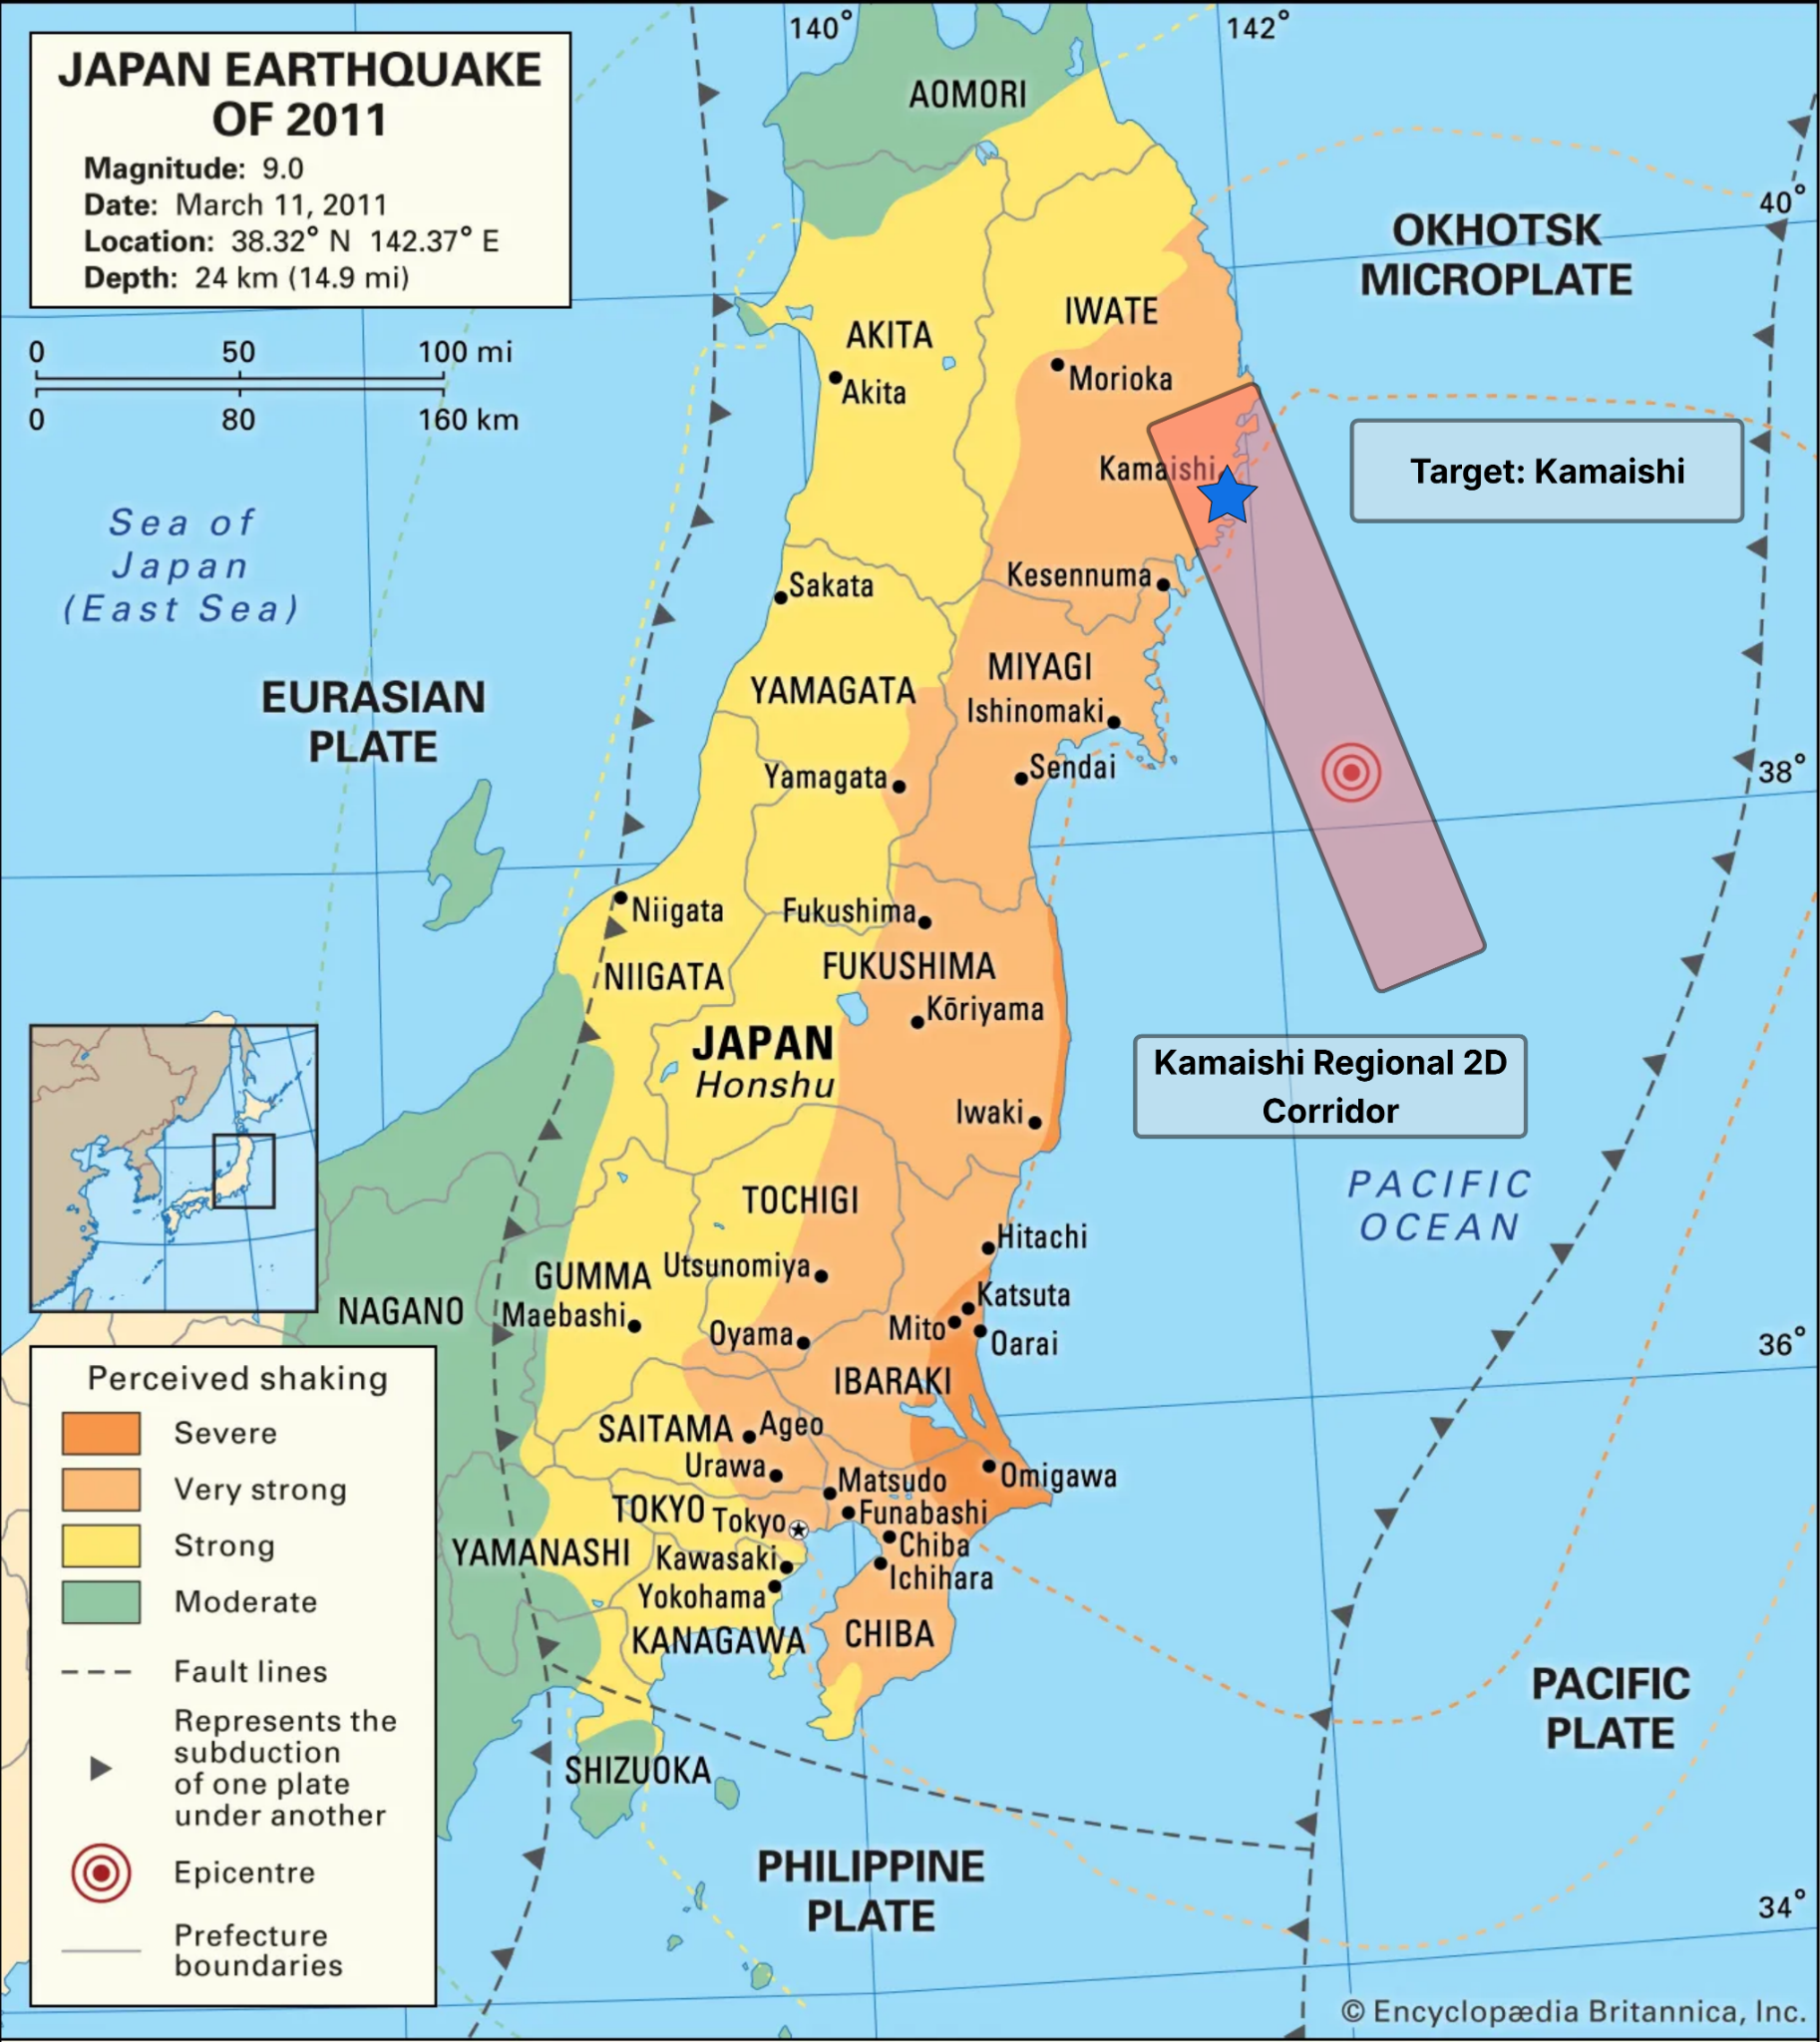
\includegraphics[width=0.88\columnwidth]{kamaishi-regional2d-corridor.png}
  \caption{Regional context for the 2011 Tōhoku tsunami showing the Kamaishi
  target and Regional2D corridor; base map adapted from Encyclopaedia
  Britannica \cite{britannica2011japan}.}
  \label{fig:corridor}
\end{figure}

\section{Coupled Modelling Framework}
% Target: approximately 220--250 words in total.
% Keep the mathematical detail selective: only the equations and numerical
% choices needed to explain the information passed between model scales.

\subsection{Regional2D Event Reconstruction}
% Describe the Tōhoku-to-Kamaishi corridor, source/terrain inputs, 2D NLSWE,
% boundary treatment, and output quantities used for coupling.
\textit{Regional2D subsection to be developed.}

\subsection{One-Way Replay Coupling and Local3D Model}
% Describe the coupling export and replay boundary; Local3D incompressible
% two-phase URANS--VOF model; k--omega SST baseline; no-defence and rigid-
% barrier cases. Do not imply two-way feedback or FSI.
\textit{Coupling and Local3D subsection to be developed.}

\begin{figure*}[t]
  \centering
  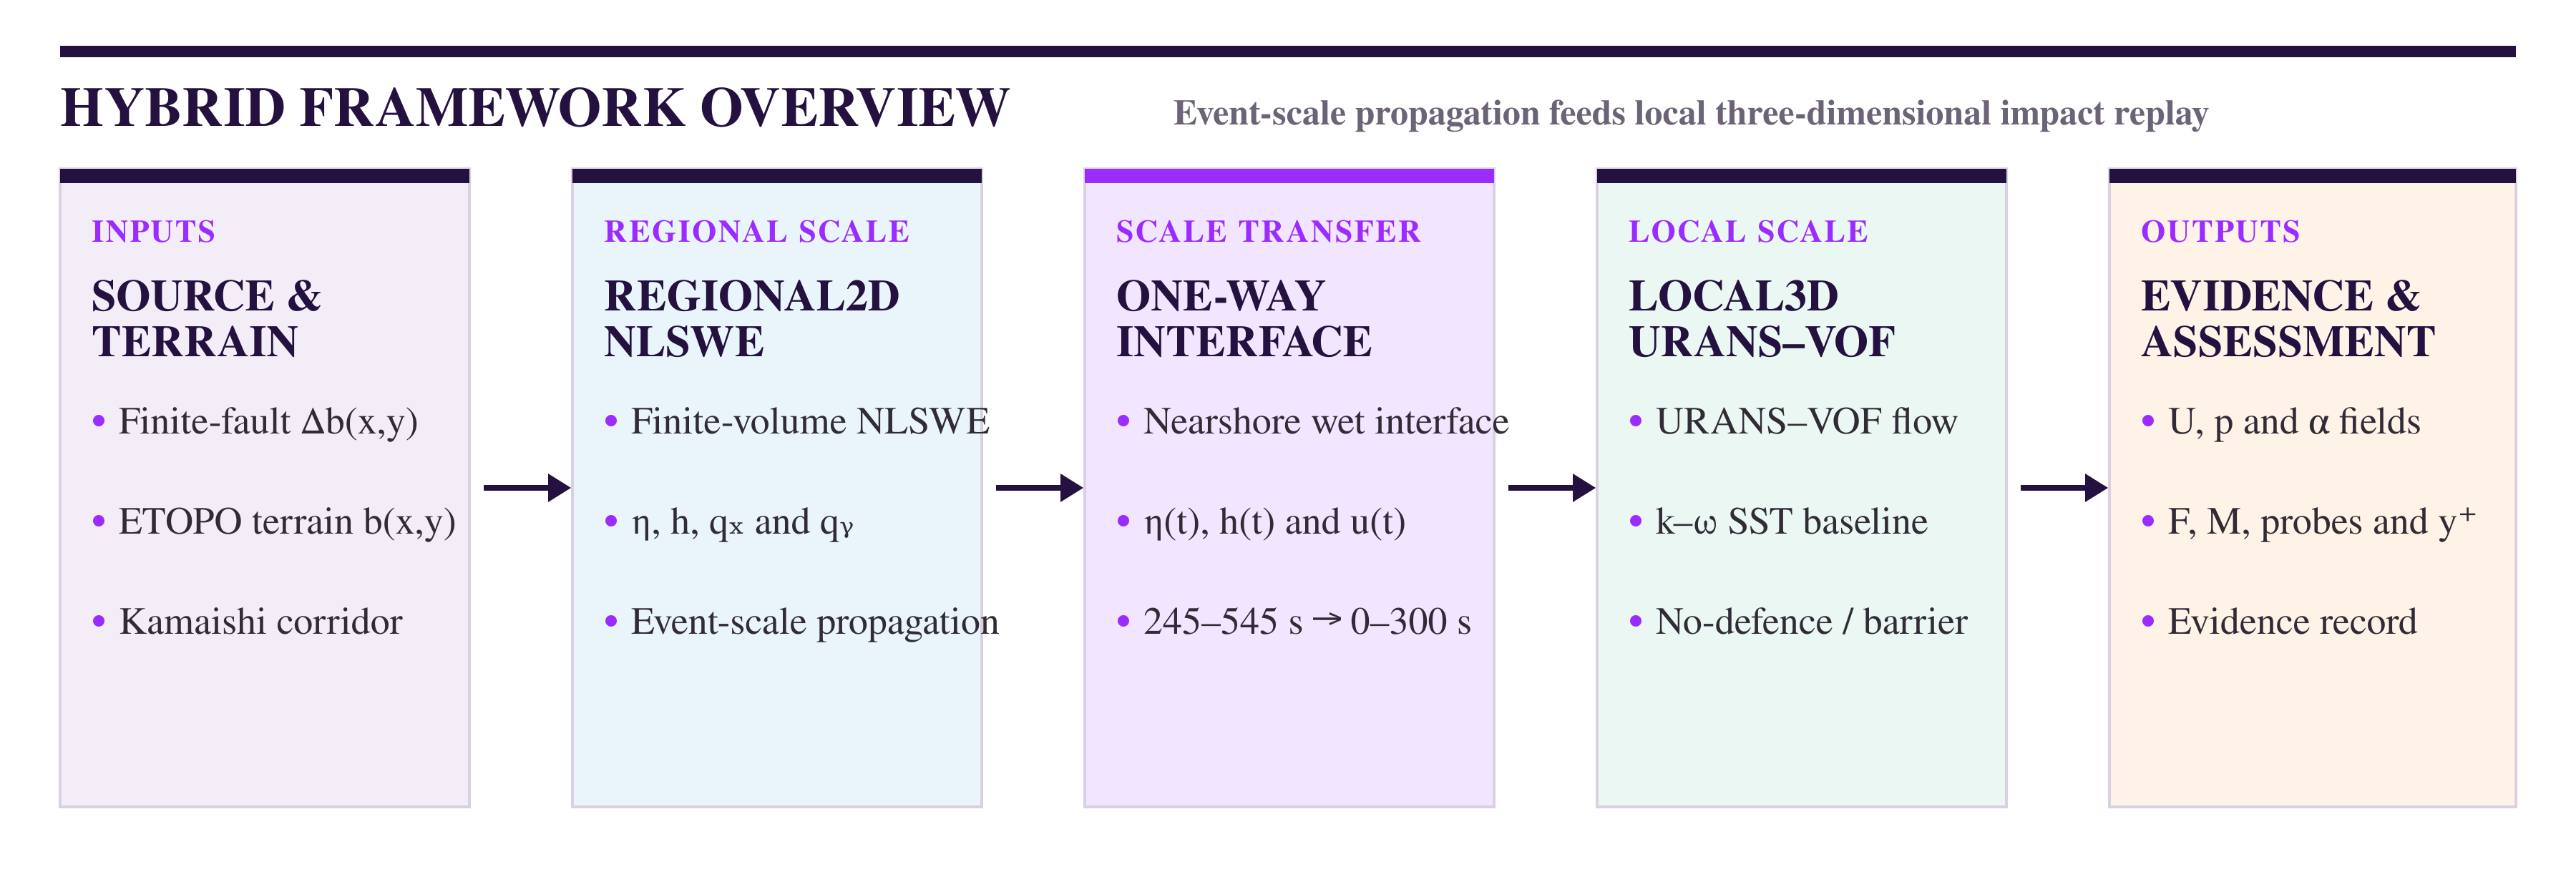
\includegraphics[width=\textwidth]{hybrid-framework-overview.png}
  \caption{One-way coupled workflow. Finite-fault and terrain data drive
  Regional2D NLSWE propagation; nearshore histories force Local3D URANS--VOF
  replay; fields and loads form the evidence outputs.}
  \label{fig:framework}
\end{figure*}

\section{Implemented Evidence and Validation Status}
% Target: approximately 150--180 words.
% Distinguish clearly between:
% - implemented: end-to-end source/terrain/Regional2D/coupling/Local3D path;
% - demonstrated or accepted: G5/G6 checks and Kamaishi replay cases;
% - incomplete: regional convergence and forcing-waveform qualification;
% - future validation: arrival time, waveform, run-up, and inundation.
\textit{Results and discussion to be developed.}

\section{Conclusion and Next Steps}
% Target: approximately 60--80 words.
% State what the framework establishes, the present evidence boundary, and the
% next validation/calibration steps. FSI, damage, and defence optimisation are
% future extensions rather than current outcomes.
\textit{Conclusion and future work to be developed.}

\appendices
\section{Original and Updated Project Plan}
\label{app:planning}

The proposal anticipated a complete event simulation, iterative
machine-learning-guided defence optimisation and subsequent structural
assessment. The updated pathway separated implementation closure from later
calibration, convergence, FSI and optimisation activities, as summarised in
Fig.~\ref{fig:planning}.

\begin{figure*}[t]
  \centering
  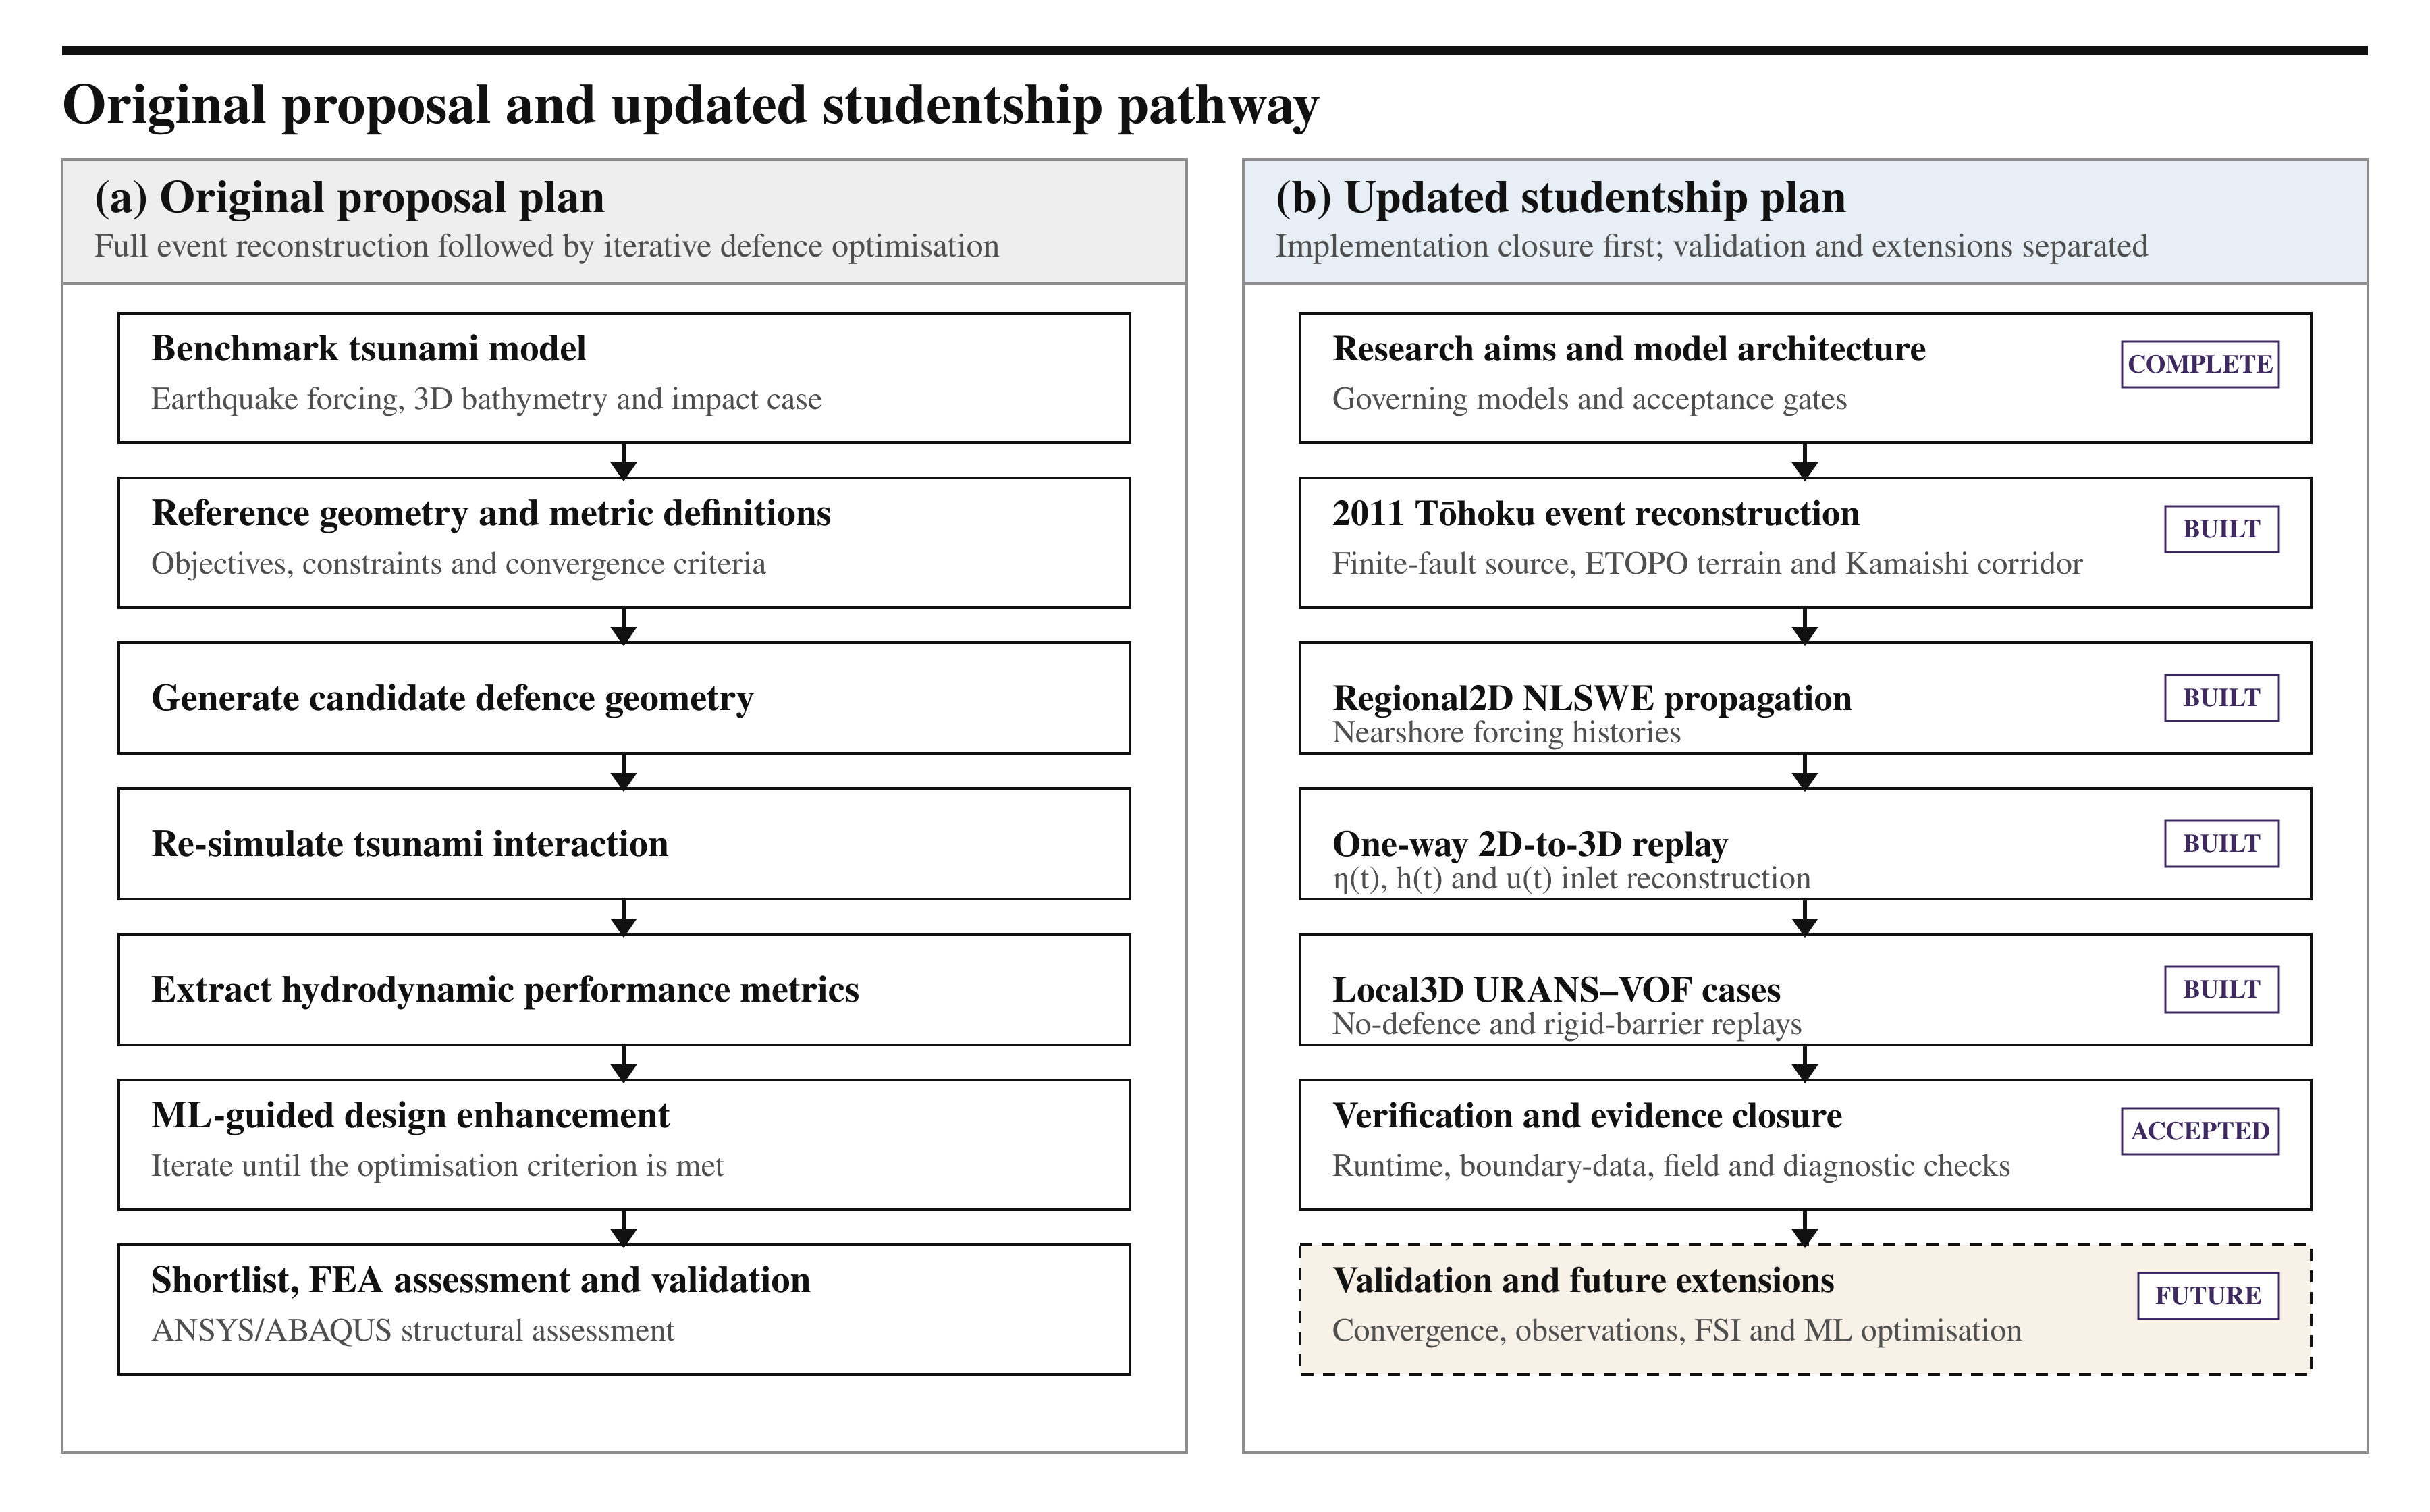
\includegraphics[width=\textwidth]{planning-overview.png}
  \caption{Comparison of the original proposal pathway with the updated
  studentship plan. The revised sequence prioritised an implemented and
  evidenced one-way Regional2D--Local3D workflow; observational calibration,
  formal convergence, FSI and optimisation remain subsequent work.}
  \label{fig:planning}
\end{figure*}

% Uncomment this block only if acknowledgements are required by the brief.
% \section*{Acknowledgment}
% The author thanks ...

\balance

% Use the report-specific subset curated from the repository-wide citation
% bank. The document also compiles while the bibliography is unavailable.
\IfFileExists{final-report.bib}{%
  \bibliographystyle{IEEEtran}
  \bibliography{final-report}
}{%
  % No bibliography is printed until final-report.bib is added.
}

\end{document}
